%  A simple AAU report template.
%  2015-05-08 v. 1.2.0
%  Copyright 2010-2015 by Jesper Kjær Nielsen <jkn@es.aau.dk>
%
%  This is free software: you can redistribute it and/or modify
%  it under the terms of the GNU General Public License as published by
%  the Free Software Foundation, either version 3 of the License, or
%  (at your option) any later version.
%
%  This is distributed in the hope that it will be useful,
%  but WITHOUT ANY WARRANTY; without even the implied warranty of
%  MERCHANTABILITY or FITNESS FOR A PARTICULAR PURPOSE.  See the
%  GNU General Public License for more details.
%
%  You can find the GNU General Public License at <http://www.gnu.org/licenses/>.
%
%  A simple AAU report template.
%  2015-05-08 v. 1.2.0
%  Copyright 2010-2015 by Jesper Kjær Nielsen <jkn@es.aau.dk>
%
%  This is free software: you can redistribute it and/or modify
%  it under the terms of the GNU General Public License as published by
%  the Free Software Foundation, either version 3 of the License, or
%  (at your option) any later version.
%
%  This is distributed in the hope that it will be useful,
%  but WITHOUT ANY WARRANTY; without even the implied warranty of
%  MERCHANTABILITY or FITNESS FOR A PARTICULAR PURPOSE.  See the
%  GNU General Public License for more details.
%
%  You can find the GNU General Public License at <http://www.gnu.org/licenses/>.
%
\documentclass[11pt,twoside,a4paper,openright]{report}
%%%%%%%%%%%%%%%%%%%%%%%%%%%%%%%%%%%%%%%%%%%%%%%%
% Language, Encoding and Fonts
% http://en.wikibooks.org/wiki/LaTeX/Internationalization
%%%%%%%%%%%%%%%%%%%%%%%%%%%%%%%%%%%%%%%%%%%%%%%%
% Select encoding of your inputs. Depends on
% your operating system and its default input
% encoding. Typically, you should use
%   Linux  : utf8 (most modern Linux distributions)
%            latin1 
%   Windows: ansinew
%            latin1 (works in most cases)
%   Mac    : applemac
% Notice that you can manually change the input
% encoding of your files by selecting "save as"
% an select the desired input encoding. 
\usepackage[utf8]{inputenc}
% Make latex understand and use the typographic
% rules of the language used in the document.
\usepackage[danish,english]{babel}
% Use the palatino font
\usepackage[sc]{mathpazo}
\linespread{1.05}         % Palatino needs more leading (space between lines)
% Choose the font encoding
\usepackage[T1]{fontenc}
%%%%%%%%%%%%%%%%%%%%%%%%%%%%%%%%%%%%%%%%%%%%%%%%
% Graphics and Tables
% http://en.wikibooks.org/wiki/LaTeX/Importing_Graphics
% http://en.wikibooks.org/wiki/LaTeX/Tables
% http://en.wikibooks.org/wiki/LaTeX/Colors
%%%%%%%%%%%%%%%%%%%%%%%%%%%%%%%%%%%%%%%%%%%%%%%%
% load a colour package
\usepackage{xcolor}
\definecolor{aaublue}{RGB}{33,26,82}% dark blue
% The standard graphics inclusion package
\usepackage{graphicx}
% Set up how figure and table captions are displayed
\usepackage{caption}
\captionsetup{%
  font=footnotesize,% set font size to footnotesize
  labelfont=bf % bold label (e.g., Figure 3.2) font
}
% Make the standard latex tables look so much better
\usepackage{array,booktabs}
% Enable the use of frames around, e.g., theorems
% The framed package is used in the example environment
\usepackage{framed}

%%%%%%%%%%%%%%%%%%%%%%%%%%%%%%%%%%%%%%%%%%%%%%%%
% Mathematics
% http://en.wikibooks.org/wiki/LaTeX/Mathematics
%%%%%%%%%%%%%%%%%%%%%%%%%%%%%%%%%%%%%%%%%%%%%%%%
% Defines new environments such as equation,
% align and split 
\usepackage{amsmath}
% Adds new math symbols
\usepackage{amssymb}
% Use theorems in your document
% The ntheorem package is also used for the example environment
% When using thmmarks, amsmath must be an option as well. Otherwise \eqref doesn't work anymore.
\usepackage[framed,amsmath,thmmarks]{ntheorem}

%%%%%%%%%%%%%%%%%%%%%%%%%%%%%%%%%%%%%%%%%%%%%%%%
% Page Layout
% http://en.wikibooks.org/wiki/LaTeX/Page_Layout
%%%%%%%%%%%%%%%%%%%%%%%%%%%%%%%%%%%%%%%%%%%%%%%%
% Change margins, papersize, etc of the document
\usepackage[
  inner=28mm,% left margin on an odd page
  outer=41mm,% right margin on an odd page
  ]{geometry}
% Modify how \chapter, \section, etc. look
% The titlesec package is very configureable
\usepackage{titlesec}
\titleformat{\chapter}[display]{\normalfont\huge\bfseries}{\chaptertitlename\ \thechapter}{20pt}{\Huge}
\titleformat*{\section}{\normalfont\Large\bfseries}
\titleformat*{\subsection}{\normalfont\large\bfseries}
\titleformat*{\subsubsection}{\normalfont\normalsize\bfseries}
%\titleformat*{\paragraph}{\normalfont\normalsize\bfseries}
%\titleformat*{\subparagraph}{\normalfont\normalsize\bfseries}

% Clear empty pages between chapters
\let\origdoublepage\cleardoublepage
\newcommand{\clearemptydoublepage}{%
  \clearpage
  {\pagestyle{empty}\origdoublepage}%
}
\let\cleardoublepage\clearemptydoublepage

% Change the headers and footers
\usepackage{fancyhdr}
\pagestyle{fancy}
\fancyhf{} %delete everything
\renewcommand{\headrulewidth}{0pt} %remove the horizontal line in the header
\fancyhead[RE]{\small\nouppercase\leftmark} %even page - chapter title
\fancyhead[LO]{\small\nouppercase\rightmark} %uneven page - section title
\fancyhead[LE,RO]{\thepage} %page number on all pages
% Do not stretch the content of a page. Instead,
% insert white space at the bottom of the page
\raggedbottom
% Enable arithmetics with length. Useful when
% typesetting the layout.
\usepackage{calc}

%%%%%%%%%%%%%%%%%%%%%%%%%%%%%%%%%%%%%%%%%%%%%%%%
% Bibliography
% http://en.wikibooks.org/wiki/LaTeX/Bibliography_Management
%%%%%%%%%%%%%%%%%%%%%%%%%%%%%%%%%%%%%%%%%%%%%%%%
\usepackage[backend=bibtex,
  bibencoding=utf8
  ]{biblatex}
\addbibresource{bib/mybib}

%%%%%%%%%%%%%%%%%%%%%%%%%%%%%%%%%%%%%%%%%%%%%%%%
% Misc
%%%%%%%%%%%%%%%%%%%%%%%%%%%%%%%%%%%%%%%%%%%%%%%%
% Add bibliography and index to the table of
% contents
\usepackage[nottoc]{tocbibind}
% Add the command \pageref{LastPage} which refers to the
% page number of the last page
\usepackage{lastpage}
% Add todo notes in the margin of the document
\usepackage[
%  disable, %turn off todonotes
  colorinlistoftodos, %enable a coloured square in the list of todos
  textwidth=\marginparwidth, %set the width of the todonotes
  textsize=scriptsize, %size of the text in the todonotes
  ]{todonotes}

%%%%%%%%%%%%%%%%%%%%%%%%%%%%%%%%%%%%%%%%%%%%%%%%
% Hyperlinks
% http://en.wikibooks.org/wiki/LaTeX/Hyperlinks
%%%%%%%%%%%%%%%%%%%%%%%%%%%%%%%%%%%%%%%%%%%%%%%%
% Enable hyperlinks and insert info into the pdf
% file. Hypperref should be loaded as one of the 
% last packages
\usepackage{listings}

\usepackage{color} %red, green, blue, yellow, cyan, magenta, black, white
\definecolor{mygreen}{RGB}{28,172,0} % color values Red, Green, Blue
\definecolor{mylilas}{RGB}{170,55,241}

\lstset{language=Matlab,%
    %basicstyle=\color{red},
    breaklines=true,%
    morekeywords={matlab2tikz},
    keywordstyle=\color{blue},%
    morekeywords=[2]{1}, keywordstyle=[2]{\color{black}},
    identifierstyle=\color{black},%
    stringstyle=\color{mylilas},
    commentstyle=\color{mygreen},%
    showstringspaces=false,%without this there will be a symbol in the places where there is a space
    numbers=left,%
    numberstyle={\tiny \color{black}},% size of the numbers
    numbersep=9pt, % this defines how far the numbers are from the text
    emph=[1]{for,end,break},emphstyle=[1]\color{red}, %some words to emphasise
    %emph=[2]{word1,word2}, emphstyle=[2]{style},    
}

\usepackage{hyperref}
\hypersetup{%
	pdfpagelabels=true,%
	plainpages=false,%
	pdfauthor={Author(s)},%
	pdftitle={Title},%
	pdfsubject={Subject},%
	bookmarksnumbered=true,%
	colorlinks=false,%
	citecolor=black,%
	filecolor=black,%
	linkcolor=black,% you should probably change this to black before printing
	urlcolor=black,%
	pdfstartview=FitH%
}% package inclusion and set up of the document
% see, e.g., http://en.wikibooks.org/wiki/LaTeX/Formatting#Hyphenation
% for more information on word hyphenation
\hyphenation{ex-am-ple hy-phen-a-tion short}
\hyphenation{long la-tex}% 
%  A simple AAU report template.
%  2015-05-08 v. 1.2.0
%  Copyright 2010-2015 by Jesper Kjær Nielsen <jkn@es.aau.dk>
%
%  This is free software: you can redistribute it and/or modify
%  it under the terms of the GNU General Public License as published by
%  the Free Software Foundation, either version 3 of the License, or
%  (at your option) any later version.
%
%  This is distributed in the hope that it will be useful,
%  but WITHOUT ANY WARRANTY; without even the implied warranty of
%  MERCHANTABILITY or FITNESS FOR A PARTICULAR PURPOSE.  See the
%  GNU General Public License for more details.
%
%  You can find the GNU General Public License at <http://www.gnu.org/licenses/>.
%
%
%
% see, e.g., http://en.wikibooks.org/wiki/LaTeX/Customizing_LaTeX#New_commands
% for more information on how to create macros

%%%%%%%%%%%%%%%%%%%%%%%%%%%%%%%%%%%%%%%%%%%%%%%%
% Macros for the titlepage
%%%%%%%%%%%%%%%%%%%%%%%%%%%%%%%%%%%%%%%%%%%%%%%%
%Creates the aau titlepage
\newcommand{\aautitlepage}[3]{%
  {
    %set up various length
    \ifx\titlepageleftcolumnwidth\undefined
      \newlength{\titlepageleftcolumnwidth}
      \newlength{\titlepagerightcolumnwidth}
    \fi
    \setlength{\titlepageleftcolumnwidth}{0.5\textwidth-\tabcolsep}
    \setlength{\titlepagerightcolumnwidth}{\textwidth-2\tabcolsep-\titlepageleftcolumnwidth}
    %create title page
    \thispagestyle{empty}
    \noindent%
    \begin{tabular}{@{}ll@{}}
      \parbox{\titlepageleftcolumnwidth}{
        \iflanguage{danish}{%
          
\includegraphics[width=\titlepageleftcolumnwidth]{figures/aau_logo_da}
        }{%
          
\includegraphics[width=\titlepageleftcolumnwidth]{figures/aau_logo_en}
        }
      } &
      \parbox{\titlepagerightcolumnwidth}{\raggedleft\sf\small
        #2
      }\bigskip\\
       #1 &
      \parbox[t]{\titlepagerightcolumnwidth}{%
      \textbf{Abstract:}\bigskip\par
        \fbox{\parbox{\titlepagerightcolumnwidth-2\fboxsep-2\fboxrule}{%
          #3
        }}
      }\\
    \end{tabular}
    \vfill
    \iflanguage{danish}{%
      \noindent{\footnotesize\emph{Rapportens indhold er frit tilgængeligt, men offentliggørelse (med kildeangivelse) må kun ske efter aftale med forfatterne.}}
    }{%
      \noindent{\footnotesize\emph{The content of this report is freely available, but publication (with reference) may only be pursued due to agreement with the author.}}
    }
    \clearpage
  }
}

%Create english project info
\newcommand{\englishprojectinfo}[8]{%
  \parbox[t]{\titlepageleftcolumnwidth}{
    \textbf{Title:}\\ #1\bigskip\par
    \textbf{Theme:}\\ #2\bigskip\par
    \textbf{Project Period:}\\ #3\bigskip\par
    \textbf{Project Group:}\\ #4\bigskip\par
    \textbf{Participant(s):}\\ #5\bigskip\par
    \textbf{Supervisor(s):}\\ #6\bigskip\par
    \textbf{Copies:} #7\bigskip\par
    \textbf{Page Numbers:} \pageref{LastPage}\bigskip\par
    \textbf{Date of Completion:}\\ #8
  }
}

%Create danish project info
\newcommand{\danishprojectinfo}[8]{%
  \parbox[t]{\titlepageleftcolumnwidth}{
    \textbf{Titel:}\\ #1\bigskip\par
    \textbf{Tema:}\\ #2\bigskip\par
    \textbf{Projektperiode:}\\ #3\bigskip\par
    \textbf{Projektgruppe:}\\ #4\bigskip\par
    \textbf{Deltager(e):}\\ #5\bigskip\par
    \textbf{Vejleder(e):}\\ #6\bigskip\par
    \textbf{Oplagstal:} #7\bigskip\par
    \textbf{Sidetal:} \pageref{LastPage}\bigskip\par
    \textbf{Afleveringsdato:}\\ #8
  }
}

%%%%%%%%%%%%%%%%%%%%%%%%%%%%%%%%%%%%%%%%%%%%%%%%
% An example environment
%%%%%%%%%%%%%%%%%%%%%%%%%%%%%%%%%%%%%%%%%%%%%%%%
\theoremheaderfont{\normalfont\bfseries}
\theorembodyfont{\normalfont}
\theoremstyle{break}
\def\theoremframecommand{{\color{gray!50}\vrule width 5pt \hspace{5pt}}}
\newshadedtheorem{exa}{Example}[chapter]
\newenvironment{example}[1]{%
		\begin{exa}[#1]
}{%
		\end{exa}
}% my new macros

\begin{document}
%frontmatter
\pagestyle{empty} %disable headers and footers
\pagenumbering{roman} %use roman page numbering in the frontmatter
%  A simple AAU report template.
%  2015-05-08 v. 1.2.0
%  Copyright 2010-2015 by Jesper Kjær Nielsen <jkn@es.aau.dk>
%
%  This is free software: you can redistribute it and/or modify
%  it under the terms of the GNU General Public License as published by
%  the Free Software Foundation, either version 3 of the License, or
%  (at your option) any later version.
%
%  This is distributed in the hope that it will be useful,
%  but WITHOUT ANY WARRANTY; without even the implied warranty of
%  MERCHANTABILITY or FITNESS FOR A PARTICULAR PURPOSE.  See the
%  GNU General Public License for more details.
%
%  You can find the GNU General Public License at <http://www.gnu.org/licenses/>.
%
\pdfbookmark[0]{Front page}{label:frontpage}%
\begin{titlepage}
  \addtolength{\hoffset}{0.5\evensidemargin-0.5\oddsidemargin} %set equal margins on the frontpage - remove this line if you want default margins
  \noindent%
  \begin{tabular}{@{}p{\textwidth}@{}}
    \toprule[2pt]
    \midrule
    \vspace{0.2cm}
    \begin{center}
    \Huge{\textbf{
      Robot Vision% insert your title here
    }}
    \end{center}
    \begin{center}
      \Large{
        - Automation and control -% insert your subtitle here
      }
    \end{center}
    \vspace{0.2cm}\\
    \midrule
    \toprule[2pt]
  \end{tabular}
  \vspace{4 cm}
  \begin{center}
    {\large
      Project Report%Insert document type (e.g., Project Report)
    }\\
    \vspace{0.2cm}
    {\Large
      Group 832%Insert your group name or real names here
    }
  \end{center}
  \vfill
  \begin{center}
  Aalborg University\\
  Electronics and IT
  \end{center}
\end{titlepage}
\clearpage
\thispagestyle{empty}
{\small
\strut\vfill % push the content to the bottom of the page
\noindent Copyright \copyright{} Aalborg University 2015\par
\vspace{0.2cm}
\noindent Here you can write something about which tools and software you have used for typesetting the document, running simulations and creating figures. If you do not know what to write, either leave this page blank or have a look at the colophon in some of your books.
}
\clearpage
\pdfbookmark[0]{English title page}{label:titlepage_en}
\aautitlepage{%
  \englishprojectinfo{
    Robot Vision LEGO Project %title
  }{%
    Robot Vision - Intelligent Manufacturing %theme
  }{%
    Spring Semester 2016 %project period
  }{%
    Group: 832 % project group
  }{%
    %list of group members
    Álvaro Pérez-Ortega\\ 
    Kenny Lund Lafon\\
    Kelvin Kjærvik Pagels\\
    Robert-Octavian Popescu\\
    Orlando Vaz
  }{%
    Dimitris Chrysostomou
  }{%
    1 % number of printed copies
  }{%
    \today % date of completion
  }%
}{%department and address
  \textbf{Electronics and IT}\\
  Aalborg University\\
  \href{http://www.aau.dk}{http://www.aau.dk}
}{% the abstract
  The aim of this project was to create predefined figurines out of LEGO Dublo blocks. Such that, a vision-based recognition and localization system using a camera and a robot arm is presented. The recognition part serves to detect the color of the blocks. Further, the positions and orientations of the needed blocks are calculated by means of image processing methods. Moreover, a translation between the image to robot frames will be done. Finally, the robot will act upon the blocks to move and pick them to construct each figurine.  
}

\cleardoublepage

\cleardoublepage
\pdfbookmark[0]{Contents}{label:contents}
\pagestyle{fancy} %enable headers and footers again
\tableofcontents
\chapter*{Preface\markboth{Preface}{Preface}}\label{ch:preface}
\addcontentsline{toc}{chapter}{Preface}
Here is the preface. You should put your signatures at the end of the preface.

\vspace{\baselineskip}\hfill Aalborg University, \today
\vfill\noindent
\begin{minipage}[b]{0.45\textwidth}
 \centering
 \rule{\textwidth}{0.5pt}\\
  Alvaro Perez Ortega\\
 {\footnotesize <aperez15@student.aau.dk>}
\end{minipage}
\hfill
\begin{minipage}[b]{0.45\textwidth}
 \centering
 \rule{\textwidth}{0.5pt}\\
  Kelvin Kjærvik Pagels\\
 {\footnotesize <kpagel15@student.aau.dk>}
\end{minipage}

\vspace{3\baselineskip}
\noindent
\begin{minipage}[b]{0.45\textwidth}
 \centering
 \rule{\textwidth}{0.5pt}\\
  Kenny Lund Lafon\\
 {\footnotesize <klafon15@student.aau.dk>}
\end{minipage}
\hfill
\begin{minipage}[b]{0.45\textwidth}
 \centering
 \rule{\textwidth}{0.5pt}\\
  Orlando Vaz\\
 {\footnotesize <obasto16@student.aau.dk>}
\end{minipage}

\vspace{3\baselineskip}

\begin{center}
\begin{minipage}[b]{0.45\textwidth}
 \centering
 \rule{\textwidth}{0.5pt}
  Robert-Octavian Popescu\\
 {\footnotesize <rpopes15@student.aau.dk>}
\end{minipage}
\end{center}

\cleardoublepage
%mainmatter
\pagenumbering{arabic} %use arabic page numbering in the mfrom workstationainmatter
\chapter{Introduction}\label{ch:introduction}

Since the Industrial Revolution, the industry has been improving itself, increasing the number of machines in factories in order to intensify the production and to reduce the effort made by the workers. However, in the last few years, the industry motto has been changing, influenced by the development of the technology. The main goal is to try to decrease the number of people working in firms, reducing, thus, the cost with manpower, and increasing the number of autonomous machines. These mechanisms are able to work without breaks for long periods with a high level of accuracy. For instance, robot arms are one of the most used instruments in factories…


The Lego Group began manufacturing the lego bricks in 1949. 
Assume that you work in a company producing Simpson figures made by Dublo brucks.

\begin{enumerate}
	\item The figures come in two sizes. One size consisting of 3x1 (or 2x1 for Maggie) Dublo bricks and one consists of 3x4 (or 2x4 for Maggie) brick.
	\item A customer can order a set of figures
\end{enumerate}

The Dublo bricks are located randomly (but not
overlapping) on a table next to a robot.

\begin{enumerate}
	\item A camera is located above the table so that all the
	bricks are within the view of the camera.
	\item Your task is to design a system which can produce
	the Simpson figures. 
\end{enumerate}

\begin{figure}[hb]
  \centering
  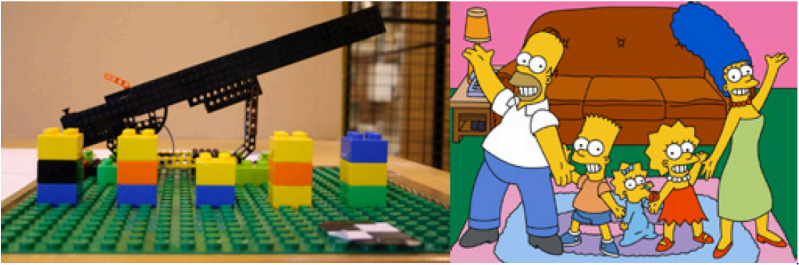
\includegraphics[width=4in]{figures/simpsonLegoBricks.png}
  \caption[Simpsons figures Lego Bricks] {A illustration of the simpsons figures with Lego Duplo Bricks}
\end{figure}

This involves among other things:
\begin{enumerate}
	\item Identifying which bricks are located on the table.
	\item Identifying the location of the bricks (e.g. the location of a
	black Dublo brick needed to build Homer)
	\item Determine the associated cost of each solution and the
	cheapest solutions.
	\item Grasping the bricks by means on a robot.
	\item Mounting the bricks on a plate or on top of other bricks
	\item Selecting the sequence in which you want to pick/place
	the bricks and build the figures
\end{enumerate}

\subsection*{Hardware}
\begin{enumerate}
	\item ADEPT Cobra
	\item Grapper
	\item Lego Blocks
	\item Logitech c920 HD Pro Webcam
\end{enumerate}

\subsection*{The Workspace} The ADEPT Cobra has to able to identify certain blocks inside its workspace. In order to so, a camera has been placed on the top of the cell where the robot is located, having a cenital point of view of the workspace.

The program will then perform an analysis of the picture in order to determine the color of the different blocks and their position in the workspace.
It is important to note that the scenario presented in this paper require different workspaces and frames.

First we have the 




\chapter{Hardware setup}\label{ch:hardware}
In order to connect to the camera and robot, a personal workstation has been used. Most of the time spent by our group was in the Robotics laboratory, where we worked and tested the ADEPT Cobra robot. We have placed inside the robot cell the camera needed to aquire images of the blocks for further processing. 

The phisical connections to the workstation were made through: 
\begin{itemize}
	\item Ethernet to the robot  
	\item USB to the camera 
\end{itemize}

\begin{figure}[hb]
\centering
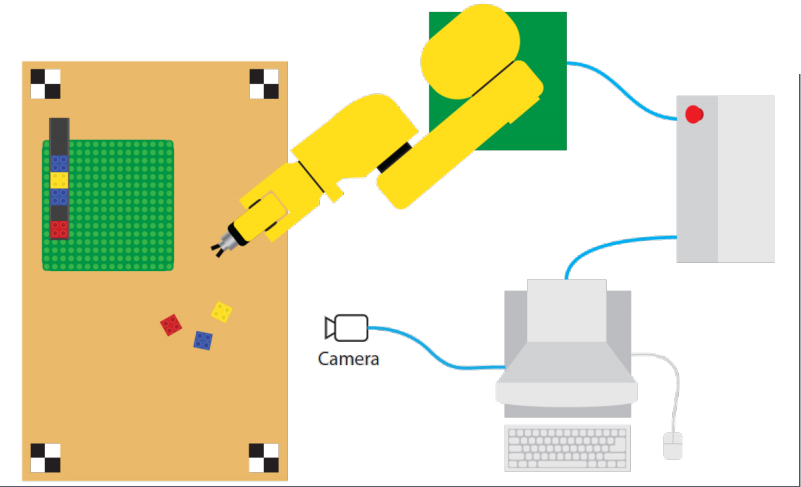
\includegraphics[width=4in]{figures/robotCellDesign.png}
\caption[robot Cell Design]
{A illustration of the robot Cell Design}
\end{figure}

The robot runs with the ADEPT Desktop program which is running on a local computer with Windows XP. This computer is connected to a switch nearby and has a static IP. Thus, we connect our workstation to that switch through a Ethernet cable and set a static IP on that port in order to connect to the ADEPT Desktop and using Matlab we send commands to the robot. Regarding the camera, it was needed to install the webcam package provided by Matlab in order to connect and properly use it. 

\chapter{Camera calibration}\label{ch:calibration}

In order to achieve the goal, the robot arm needs to be combined with a camera which will provide important information to detect the correct position of the bricks. However, the use of this camera demanded a calibration which was done with a checkerboard. This calibration was essential in order to find the intrinsic and extrinsic parameters of the camera which were useful to make some transformations between frames. Besides, the calibration was also used to undistort images taken by the camera which were used to detect the position of the blocks.

The calibration of the camera was performed using the \textit{Camera Calibration Toolbox} and it was based on thirty different pictures of the checkerboard. In each image, four different corners were selected (the first corner was the origin) as well as defined the size of the each square. This process was repeated in the same order for all pictures to be able to calibrate the camera. After selecting all the corners, it was necessary to calibrate the camera using the data colected from the pictures. The first step of this calibration computes a closed-form solution for the calibration parameters without considering the lens distortion. This step is followed by a nonlinear optimization where the main goal is to minimize the total reprojection error over all the calibration parameters (intrinsic and extrinsic). This optimization is done iteratively based on the gradient descent method and, at the end, the result is a set of variables which describe every parameter. 

In addition, the calibration results also show the errors associated with some variables which allow to understand the quality of the calibration. Moreover, using the plot of the errors provided by the calibration, it becomes easy to compare the error between pictures and, based on this information, some pictures were eliminated (the ones with the biggest error values). After eliminating the worst pictures, the image corners were recomputed automatically using the function \textit{Recomp. Corners} and then the \textit{Calibration} function was applied in order to get new parameters with a small error.

Furthermore, the camera calibration was also used in the undistortion process to undistort the background image and the images with bricks. This process was essential to remove the deformation in the external areas and, thus, obtain the best position values of the blocks. \par


\subsection*{Intrinsic and Extrinsic Parameters}
The parameters provided by the calibration of the camera can be used to make transformations between frames which is useful to calculate the correct position of the bricks. These parameters can be divided in two different groups: the intrinsic and the extrinsic. The intrinsic parameters are related to the camera (equation \ref{intrinsic}), for instances, the position of the principal point, the skew parameter (is zero because the axis are orthogonal) and the focal length. Using these parameters it is possible to combine the coordinates of the camera frame with the ones in the picture (pixels). The extrinsic parameters are the ones responsible for the relation between the world coordinates and the camera coordinates as is possible to see in \ref{extrinsic}.

\begin{align} 
\label{intrinsic}
\begin{bmatrix}
    \textit{u} \\ 
    \textit{v} \\
    \textit{w} 
\end{bmatrix}
=
\begin{bmatrix}
    \textit{f}  & 0 & p_{x} & 0\\
    0   &  \textit{f} & p_{y} & 0  \\
    0 & 0 & 1 & 0 
\end{bmatrix}
\begin{bmatrix}
   x_{s}\\
   y_{s}\\
   z_{s}\\
	1
\end{bmatrix}
\text{  , K}
=
\begin{bmatrix}
    \textit{f}  & 0 & p_{x} & 0\\
    0   &  \textit{f} & p_{y} & 0  \\
    0 & 0 & 1 & 0 
\end{bmatrix}
\end{align}

\begin{align} 
\label{extrinsic}
\begin{bmatrix}
   x_{s}\\
   y_{s}\\
   z_{s}\\
	1
\end{bmatrix}
=
\begin{bmatrix}
    \textit{R}  & \textit{T}
\end{bmatrix}
\begin{bmatrix}
   X_{w}\\
   Y_{w}\\
   Z_{w}\\
	1
\end{bmatrix}
\end{align}

Based on the relations between frames, it is possible to simplify the calculations associating the image coordinates with the world coordinates. The relation is made through a projective matrix ($3\times 4$ matrix) which is a result of the product between the intrinsic ($3\times 3$ matrix) and extrinsic ($3\times 4$ matrix) matrices.

\begin{align} 
\begin{bmatrix}
    \textit{u} \\ 
    \textit{v} \\
    \textit{w} 
\end{bmatrix}
=
\textit{K}
\begin{bmatrix}
    \textit{R}  & \textit{T}
\end{bmatrix}
\begin{bmatrix}
   X_{w}\\
   Y_{w}\\
   Z_{w}\\
	1
\end{bmatrix}
=
\textit{P}
\begin{bmatrix}
   X_{w}\\
   Y_{w}\\
   Z_{w}\\
	1
\end{bmatrix}
\end{align}

The projective matrix is a $3\times 4$ matrix which means that it is not invertible. However, it is possible to assume that \textit{Z} is always zero because the blocks are in the \textit{XY} plane and thus the third column of the projective matrix will be multiplied by zero. So, it is possible to ignore the third column of the projective matrix and the third row of the matrix with the world coordinates.

\begin{align} 
\begin{bmatrix}
    \textit{u} \\ 
    \textit{v} \\
    \textit{w} 
\end{bmatrix}
=
\textit{P}
\begin{bmatrix}
   X_{w}\\
   Y_{w}\\
	1
\end{bmatrix}
\end{align}

As a result, \textit{P} can be represented as $3\times 3$ matrix which means that it is invertible, as it is possible to observe in \ref{invertible}. 

\begin{align}
\begin{bmatrix}
   X_{w}\\
   Y_{w}\\
	1
\end{bmatrix} 
=
\textit{P}^{-1}
\begin{bmatrix}
    \textit{u} \\ 
    \textit{v} \\
    \textit{w} 
\end{bmatrix}
\label{invertible}
\end{align}


\chapter{Frames}\label{ch:frames}
A coordinate system is a reference framework that defines the position in either two- or three-dimensional space. In this chapter, the relationship between the coordinate system for the world and for the Cobra will be taken into account. A relationship between the robot and the world coordinates allows to go from the world coordinate to the robot. In figure \ref{fig:check_coordrobottoworld}, it is shown that the world coordinate is rotated and translated relative to the robot frame. 
\begin{figure}[hb]
  \centering
  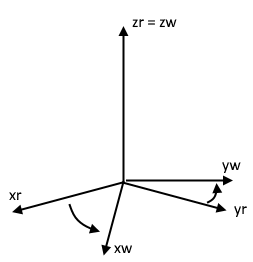
\includegraphics[width=3in]{figures/coordrobottoworld.png}
  \caption[Checkerboard and coordinate with robot to world] {Checkboard and coordinate with robot to world}
  \label{fig:check_coordrobottoworld}
\end{figure}

To transform the coordinate system from Robot to the World coordinates some calculations are needed. The following equation shows the relationship between the robot frame and the world frame.
\begin{align*}
\begin{bmatrix}
x_r \\
y_r \\
z_r \\
1 
\end{bmatrix}
= \underbrace{\begin{bmatrix}
a & b & x & c \\
d & e & x & f \\
g & h & x & i 
\end{bmatrix}}_{\text{R | T}}
\begin{bmatrix}
x_w \\
y_w \\
z_w\\
1 
\end{bmatrix}
\end{align*}
We assume that the z axis is on the same axis in both robot and world coordinate. The reason for this are that everything is measured in the XY plane. Therefore the above equation can we written as: 
\begin{align}
\begin{bmatrix}
x_r \\
y_r \\
1 
\end{bmatrix}
= \underbrace{\begin{bmatrix}
a & b & c \\
d & e & f \\
g & h & i 
\end{bmatrix}}_{\text{    R   | T}}
\begin{bmatrix}
x_w \\
y_w \\
1 
\end{bmatrix}
\label{eq:world_to_robot}
\end{align}

In order to find the coordinates $(x_r,y_r,z_r)$ in the robot frame, the matrix [R | T] and the coordinates in the world frame $(x_w,y_w,z_w)$ must be known. However, in this situation, only  the coordinates in the world frame were known. So, in order to find the robot coordinates in equation \ref{eq:world_to_robot}, the matrix [R | T] needs to be calculated. An easy way to find the solution of this issue would be to solve the [R | T] matrix as a system of equations. So that, if one point is known in the robot frame and in the world one, we will have three equations with nine unknowns. It is possible to observe these three equations with nine unknown between \ref{eq:system_of_equations1} and \ref{eq:system_of_equations2}.
 
\begin{align}
\label{eq:system_of_equations1}
x_r &= a\cdot x_w + b\cdot y_w + c \\
y_r &= d\cdot x_w + e\cdot y_w + f \\
1 &= g\cdot x_w + h\cdot y_w + i
\label{eq:system_of_equations2}
\end{align}
In order to solve this system, six more equations would be necessary to get the values of the [R | T] matrix. As a consequence, two more points would be essential to find nine different equations with nine unknown. 

The coordinates in the robot and world frames are measured by putting the robot manually at three different positions. To find the values of these points in the robot frame, a checkerboard is used as shown in figure \ref{fig:checkerboard}. 

\begin{figure}[h]
  \centering
  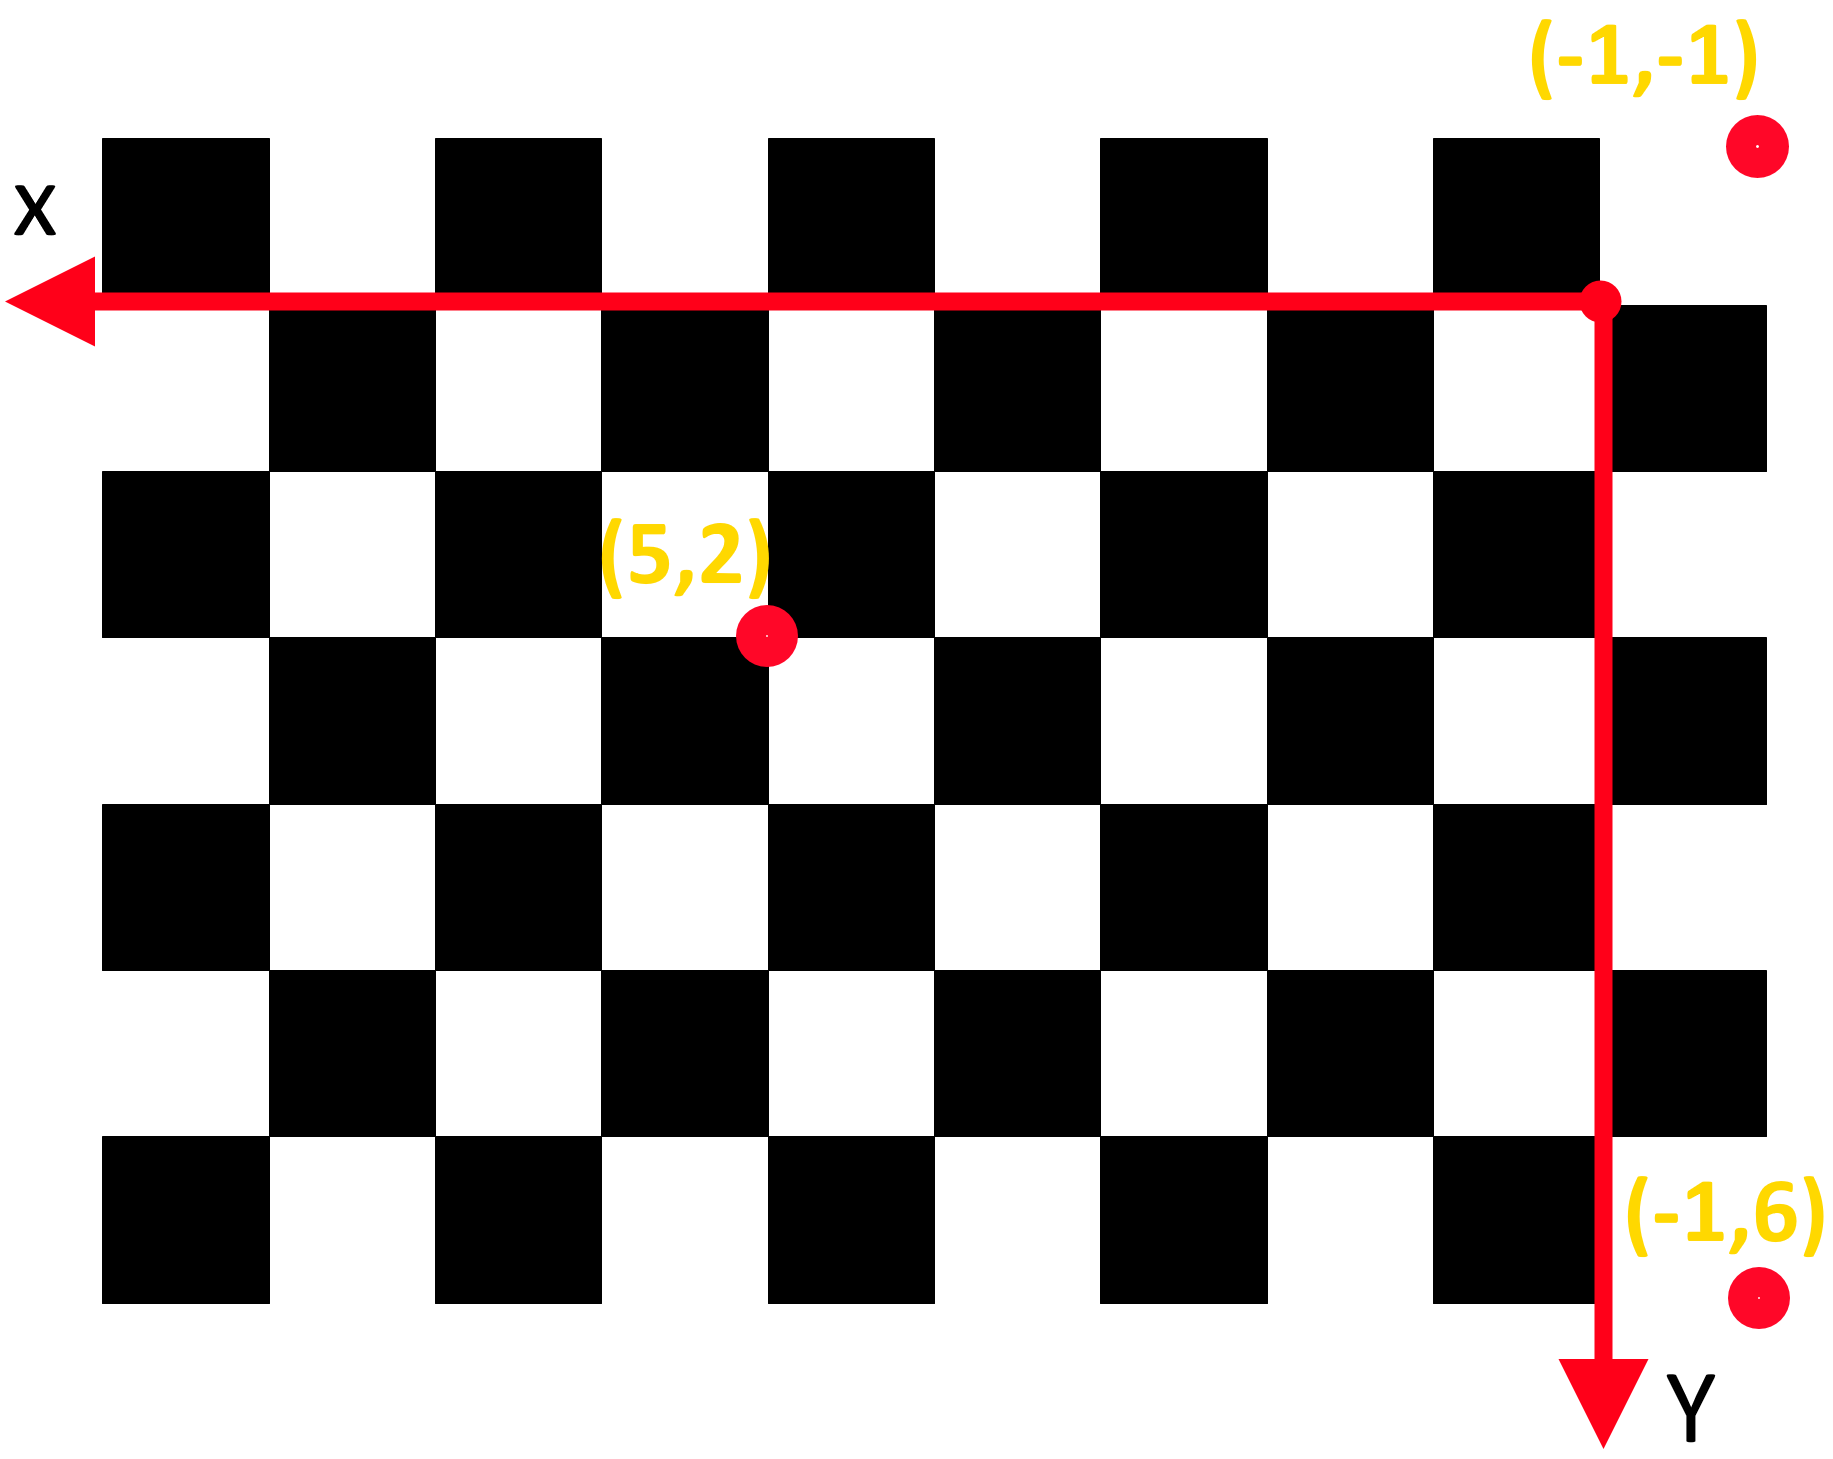
\includegraphics[width=2in]{figures/pattern.png}
  \caption[Checkerboard pattern] {Checkerboard pattern}
  \label{fig:checkerboard}
\end{figure}

The origin (0,0) is already known and from that it is possible to choose other two different positions. When these points are found, the nine different equations can be solved. The values of these three points are:

\begin{table}[h]
\begin{tabular}{| c | c | c | c |}
\hline
   & Point 1 & Point 2 & Point 3 \\
   \hline
  World & 28*[-1\quad -1] & 28*[-1\quad 6] & 28*[5\quad 2] \\
  Robot & [239.484\quad 198.714] & [233.953\quad 398.995]   & [408.578\quad 287.651] \\
  \hline
\end{tabular}
\end{table}

The 9 different equations will then be:
\begin{align*} 
p_1(x_r) &= a\cdot p_1(x_w) + b\cdot p_1(y_w) + c \\
p_1(y_r) &= d\cdot p_1(x_w) + e\cdot p_1(y_w) + f \\
1 &= g\cdot p_1(x_w) + h\cdot p_1(y_w) + k \\
p_2(x_r) &= a\cdot p_2(x_w) + b\cdot p_2(y_w) + c\\
p_2(y_r) &= d\cdot p_2(x_w) + e\cdot p_2(y_w) + f \\
1 &= g\cdot p_2(x_w) + h\cdot p_2(y_w) + k \\
p_3(x_r) &= a\cdot p_3(x_w) + b\cdot p_3(y_w) + c \\
p_3(y_r) &= d\cdot p_3(x_w) + e\cdot p_3(y_w) + f \\
1 &= g\cdot p_3(x_w) + h\cdot p_3(y_w) + k
\end{align*}
By solving these equations the [R | T] matrix is:
\begin{align*}
\text{(R|T)} = 
\begin{bmatrix}
1.0206 & -0.0282 & 267.2713 \\
0.0185 & 1.0218 & 227.8426 \\
0 & 0 & 1.0000 
\end{bmatrix}
\end{align*}



\chapter{Block}\label{ch:block_recognition}


In order to complete the block recognition part of our project, we had to go through 3 main steps, the background substraction, color recognition and edge detection.

\begin{flushleft}
Background substraction
\end{flushleft}



\begin{flushleft}
Color recognition
\end{flushleft}


 	Once the background substracted, we obtained the color of the blocks experimentaly by using the tool 'Pixel region' in Matlab. A color can be expressed with values between 0 and 255 for its primary colors, red, green and blue. Thus, for each block, we placed the 'Pixel region' tool on it to get a range for the RGB parameters.\par
\begin{flushleft}
Let's take an example with the yellow block.
\end{flushleft} \par

\begin{figure}[hb]
  \centering
  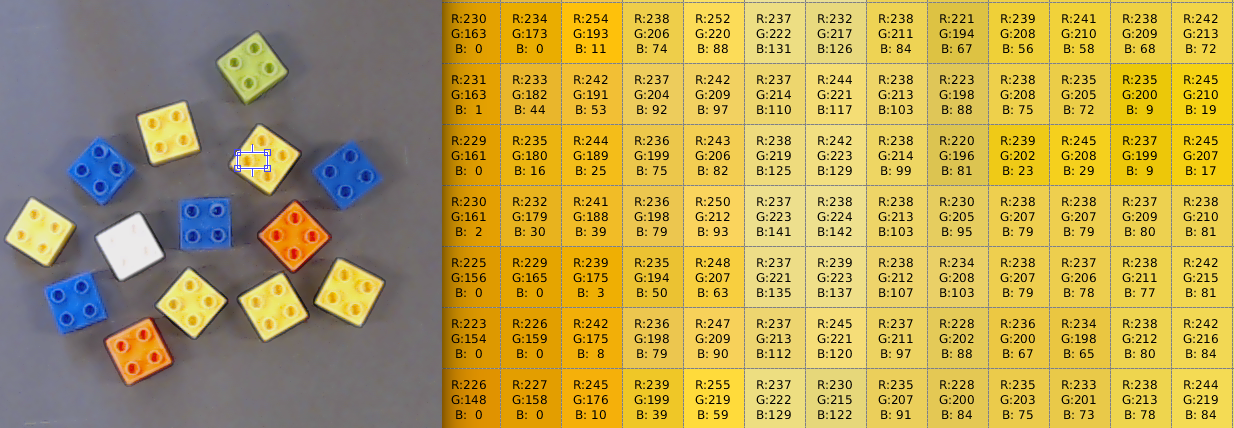
\includegraphics[scale=0.3]{figures/Thres_Y_manualy2.png}
  \caption[LABEL] {CAPTATION TEXT}
\end{figure}

Here the result by experiment gives us more or less a range of R = [], G = [] and B = [] for the RGB parameter. This parameter is then used to check in a loop that every pixel of the image are within the ranges.\par
In the image below the pixels being in the RGB parameter are highlighted in white while the others are put into black. 

\begin{figure}[hb]
  \centering
  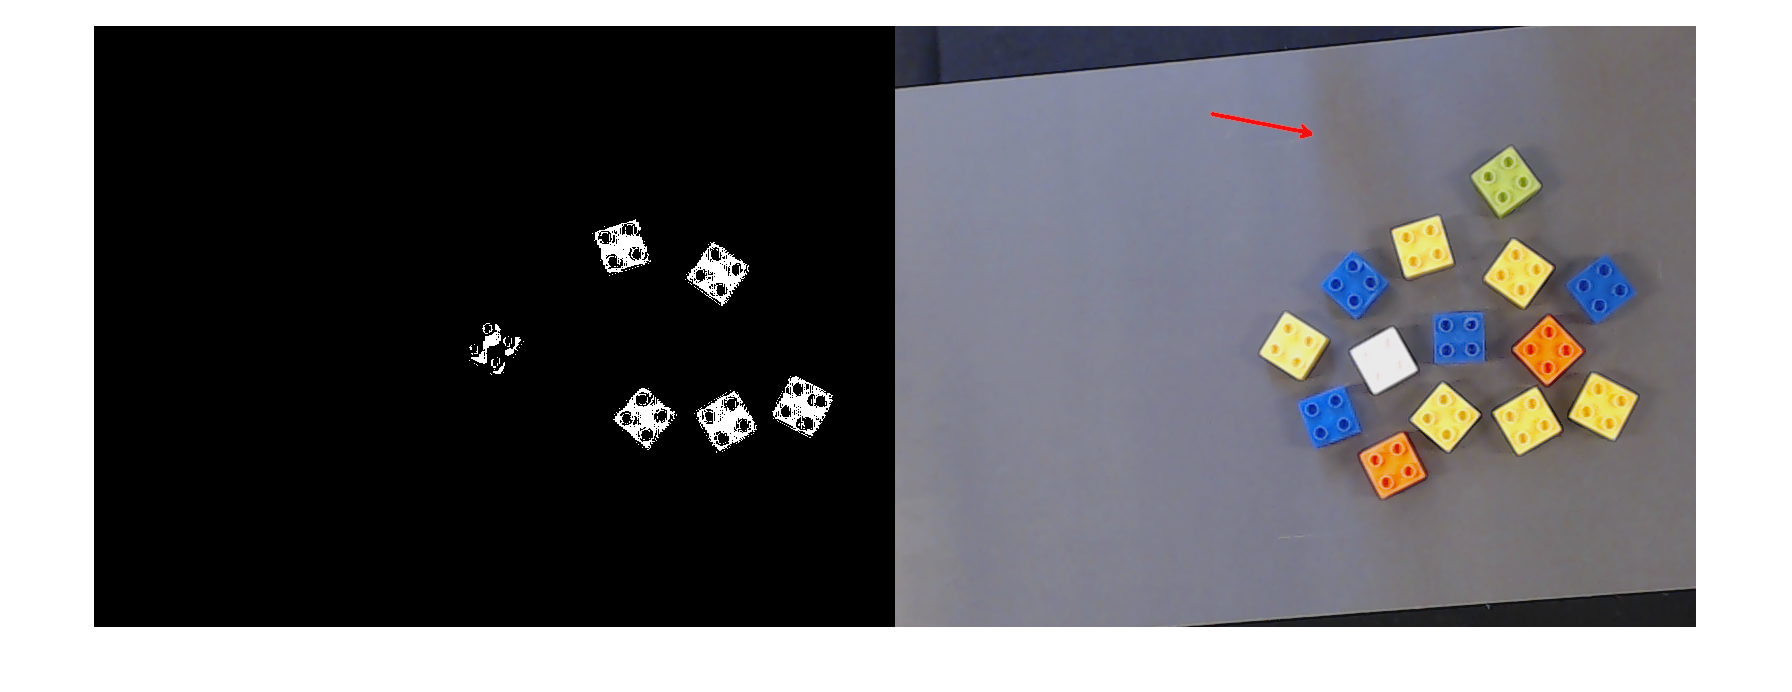
\includegraphics[scale=0.3]{figures/Thres_Y_bad2.png}
  \caption[LABEL] {CAPTATION TEXT}
\end{figure}
  
\begin{flushleft}
We can see that the 6 yellow blocks are detected. However, the one on the left is partially detected. This is the consequence of the different lights in the robot cell. The RBG range was define on a block placed in zone of shadow (see the red arrow on the picture).
\end{flushleft}  
\par

\begin{flushleft}
Thus, the color recognition was redefined taking into account the different light inside the robot cell. All the yellow blocks are now detected.
\end{flushleft}


\begin{figure}[hb]
  \centering
  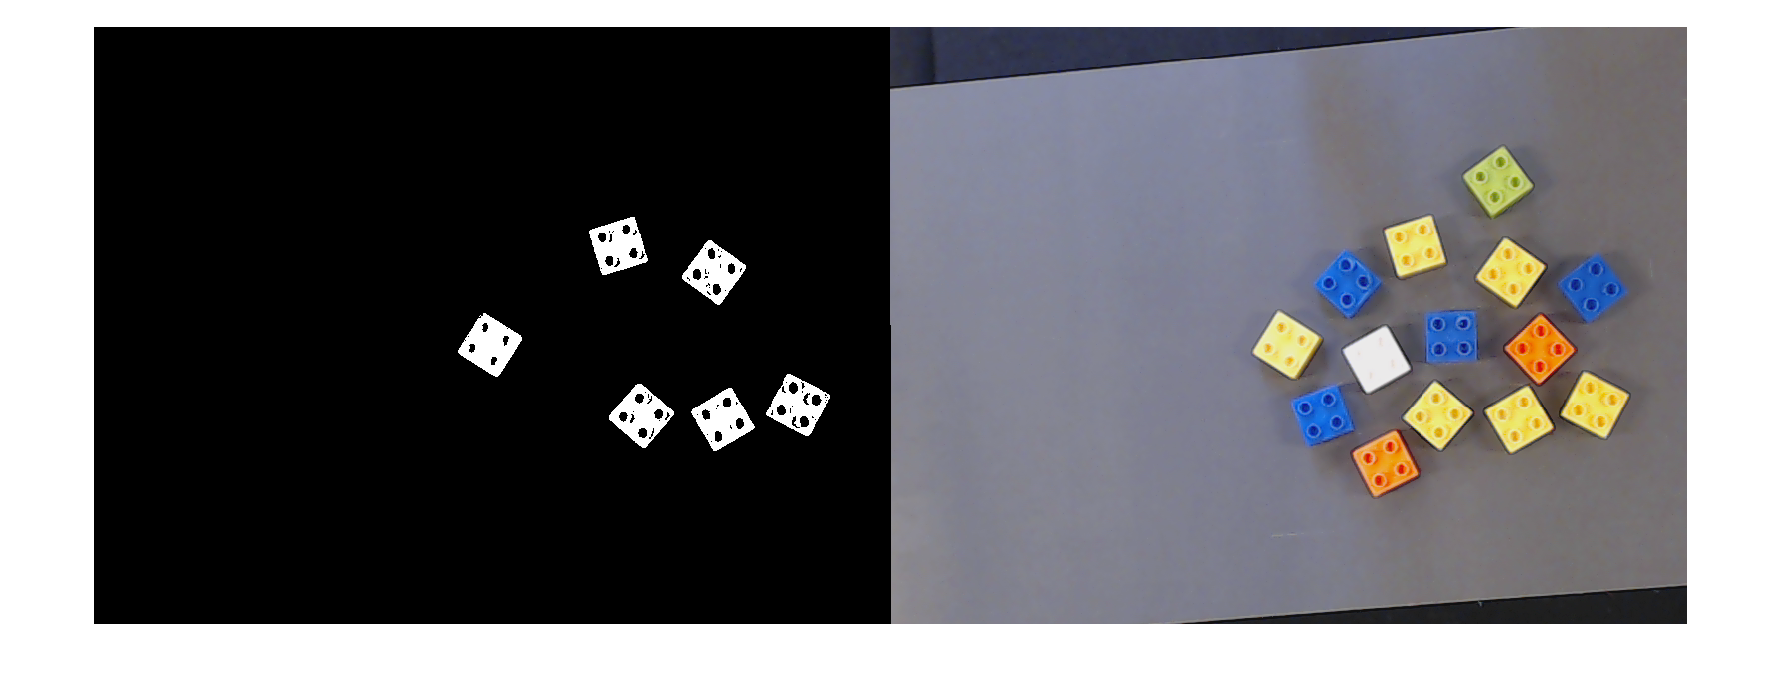
\includegraphics[scale=0.3]{figures/Thres_Y_good.png}
  \caption[LABEL] {CAPTATION TEXT}
\end{figure}

\begin{flushleft}
An other solution would have been to set up a source of light inside the cell to have more precise ranges for the colors resulting in more robust system.
\end{flushleft}



 \begin{flushleft}
 Edge detection
 \end{flushleft}
 
	There is different methods to detect the edges in an image. To pick the best one for our application, we played around the Canny, log, Prewitt, Roberts, Sobel and zerocross methods and their parameters as the threshold, direction and the standard deviation of the filter.

............(present here some of them? )

As a result of the tests done, we chose to use the Canny method with a standard deviation of 5.

...............(insert 4 pictures here? without sigma/ with 5/ with >/ with <)
\chapter{Building methods}\label{ch:building_methods}

Two different approaches for building the figures have been addressed on the project. They will be refered through the text as \textit{"On the fly"} and \textit{"Regular"} construction.

As it has been explain during the progress of this document, the \textit{"Regular"} construction consists of the following steps:
\begin{enumerate}
	\item Loading intrinsic and extrinsic parameters.
	\item Create projective matrix by using these parameters.
	\item Taking picture of the current workspace.
	\item Crop workspace image. 
	\item Substract background.
	\item Threshold (segmentation) and filter image.
	\item Calculate edges and choose the "biggest" block.
	\item Calculate the centroid and the angle, based on the slop of the block's side.
	\item Translate the image coordinates of the chosen block to world and the robot coordinates.
	\item Move the robot to the calculated position with its respective angle and pick the block.
	\item Move the robot to the building board and drop the block.
	\item Repeat steps 3-11 until the selected figure is finished. Note that the height of the position in the building board will be different depending on how many iterations have been carried out before.
\end{enumerate}

The "On the fly" construction differs a bit in some of the steps with the "Regular" one.
For starters, this second form of building will only take \textbf{one} picture for figure. This results in a faster construction since taking a new picture and making the whole process to calculate new positions of the blocks every time takes quite a bit of time.
However, this sort of process introduces a new problem to the table, since we are choosing the block that is going to be picked based on the maximum area and, in some cases, the same color will have to be picked twice.

For this reason a "color counter" has been added during this method, keeping track of how many times a certain color has been picked and therefore calculating the position of the desired block as the relative maximum area with respect to the counter. I.e.: If one color has to be picked more than once, the block with the second biggest area would be picked the second time, the one with the third biggest area would be picked the third time, and so on. 

On the other hand, even though the "On the fly" construction is significantly faster, it is also way less \textbf{robust}. This is due to the fact of taking only one picture for each figure construction. A compromise between speed and robustness should be achieved in a real scenario, since new blocks can be add to the workspace while a figure is being constructed or even considering the fact that the first (and only) picture is taken in the process might happen to be of not very good quality (blurred).

%\chapter{Chapter 2 name}\label{ch:ch2label}
Here is chapter 2. If you want to leearn \todo{I think this word is mispelled} more about \LaTeXe{}, have a look at \cite{Madsen2010}, \cite{Oetiker2010} and \cite{Mittelbach2005}.
\missingfigure{We need a figure right here!}
\chapter{Conclusion}\label{ch:conclusion}
Our conclusion.
\printbibliography[heading=bibintoc]
\label{bib:mybiblio}
\end{document}